\section{Results}\label{sec:results}

\subsection{Agent Type}\label{subsec:agent-type}
The average rewards by agent type can be seen in \autoref{fig:rewards-by-agent}.
Unfortunately, none of the agents were able to do as well as the controller used by the
CPT\@.
Additionally, all agents performed as bad or worse as a simple random controller!
It is possible that this problem is complex enough that the models needed more time
to train, but no significant additional gains were made when training for over 12,000
episodes, so there appears to be something wrong.

\begin{figure}[!ht]
    \centering
    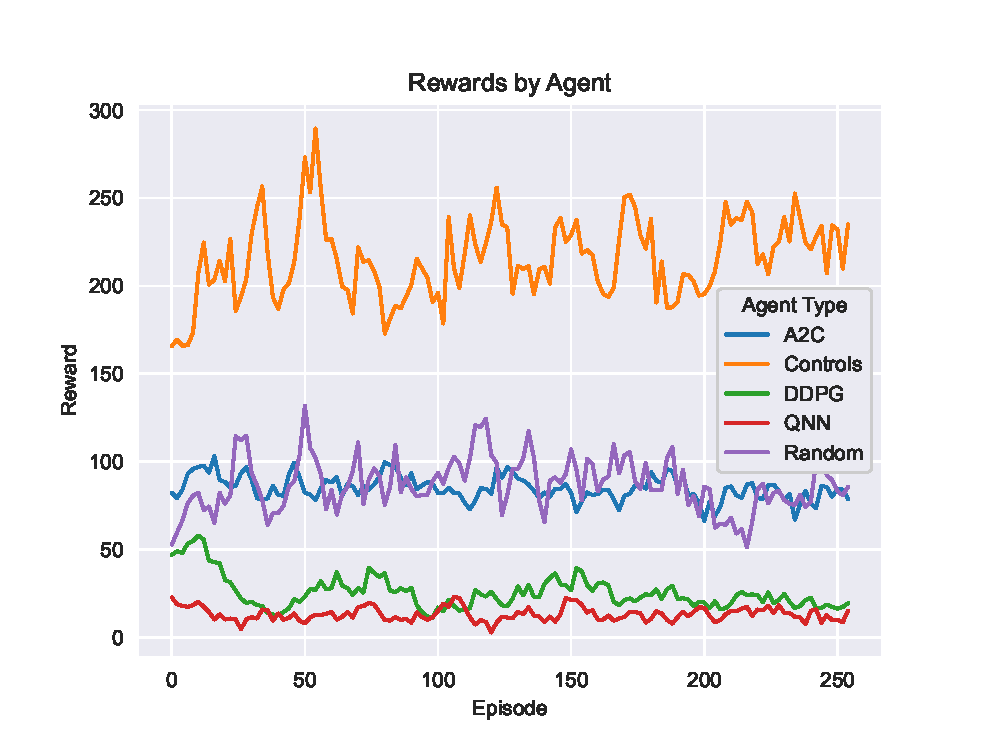
\includegraphics[scale=0.5]
    {./figures/rewards-by-agent}
    \caption{
        Rewards by agent type.
        The x-axis is the episode, while the y-axis is the reward.
    }
    \label{fig:rewards-by-agent}
\end{figure}

Interestingly, the A2C agents seems to perform the best out of all the agents used.
DDPG seems to perform second best, while QNN performs the worst.
Further work should be done to determine why these agents aren't improving and what
changes need to be made to improve them.
The average reward for each agent is shown in \autoref{tab:agent-average-reward}.

\begin{table}[!htbp]
    % increase table row spacing, adjust to taste
    \renewcommand{\arraystretch}{1.3}

    \caption{The average rewards by agent type.}
    \label{tab:agent-average-reward}

    \centering
    \begin{tabular}{|c|c|}
        \hline
        Agent    & Average Reward \\
        \hhline{|=|=|}
        A2C      & 84.77          \\
        \hline
        Controls & 216.75         \\
        \hline
        DDPG     & 25.05          \\
        \hline
        QNN      & 13.04          \\
        \hline
        Random   & 87.68          \\
        \hline
    \end{tabular}
\end{table}

\subsection{Memory Type}\label{subsec:memory-type}
The loss by memory type is displayed per agent type in \autoref{fig:loss-by-memory}.
Specifically, the loss for the actor is used in the case of A2C and DDPG, while QNN
simply displays ``loss'' since it itself is the actor.

\begin{figure}[!ht]
    \centering
    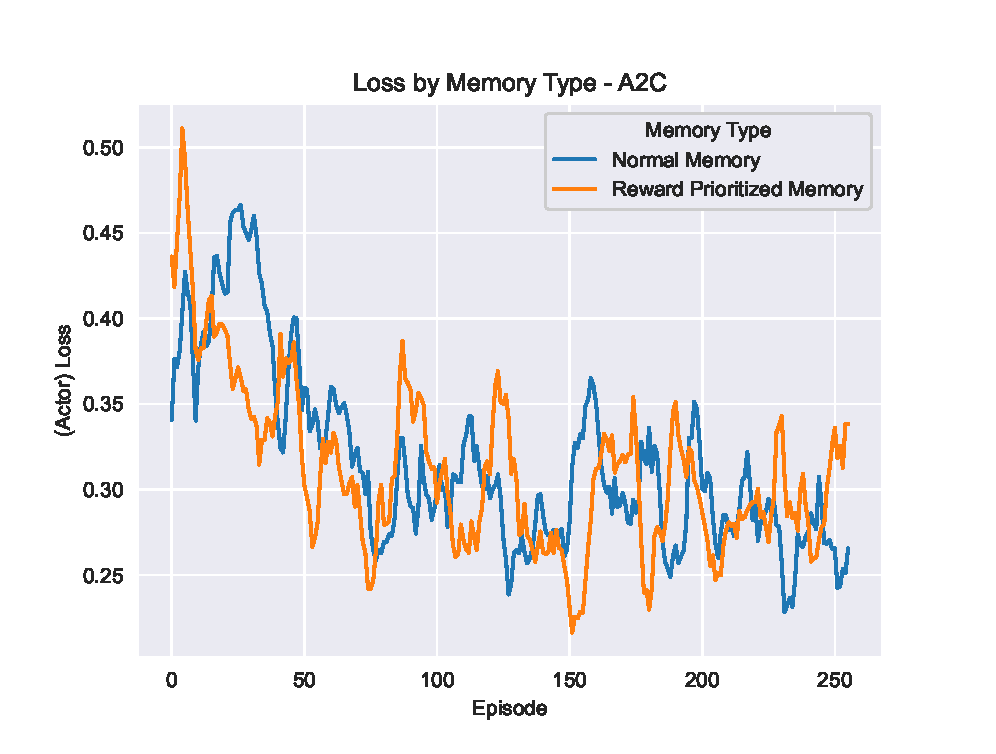
\includegraphics[scale=0.5]
    {./figures/memory/loss-by-memory-A2C}
    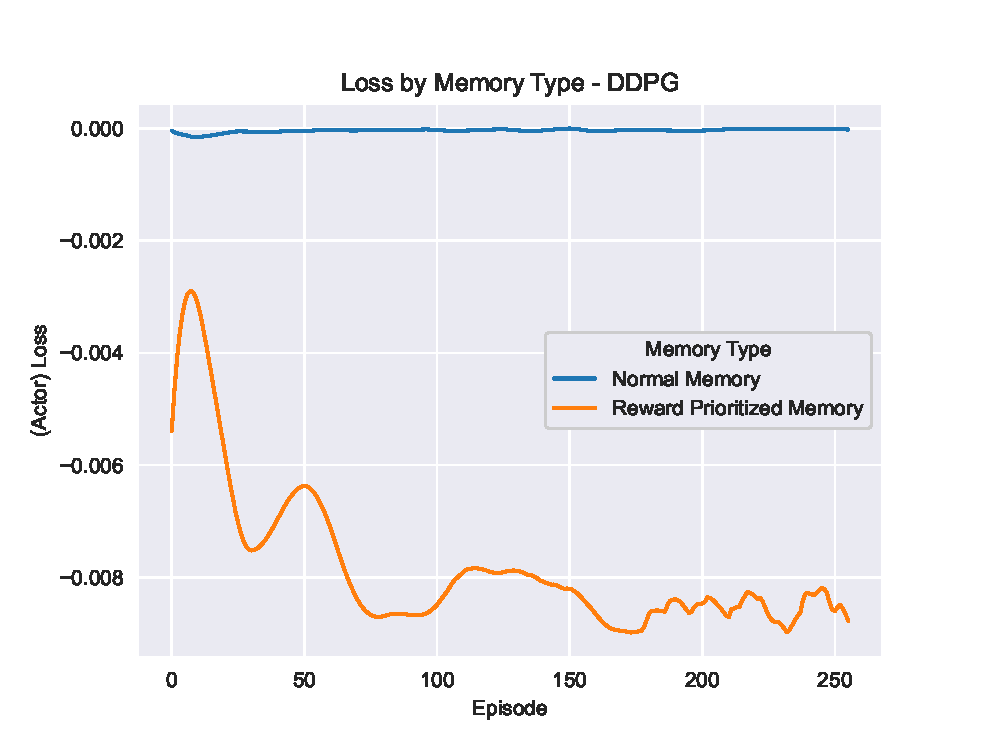
\includegraphics[scale=0.5]
    {./figures/memory/loss-by-memory-DDPG}
    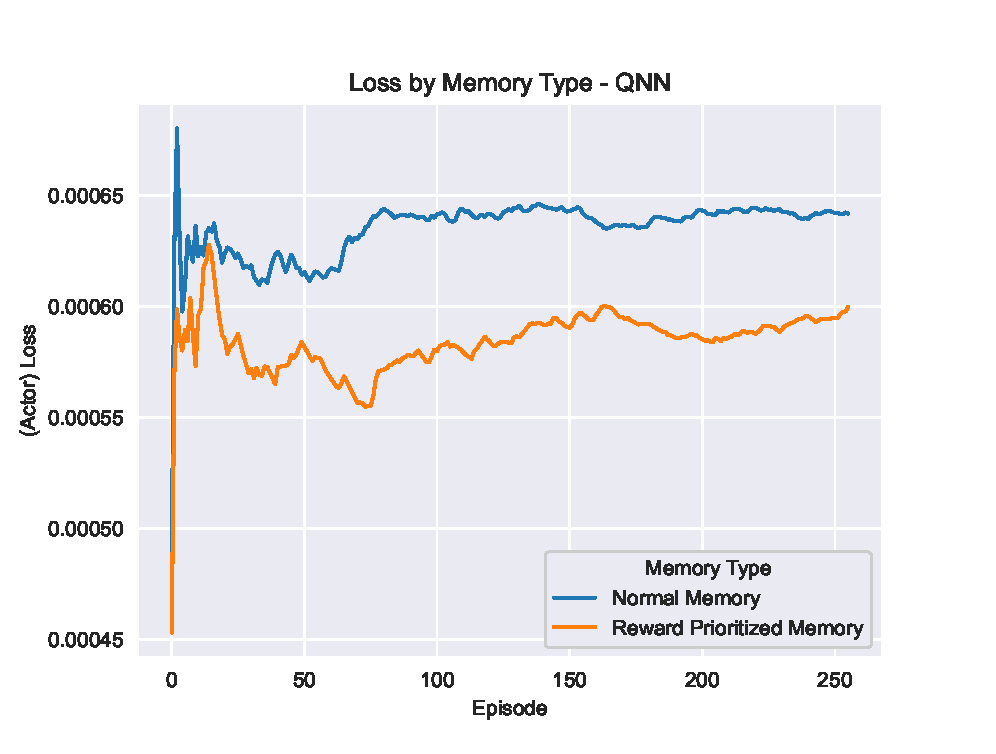
\includegraphics[scale=0.5]
    {./figures/memory/loss-by-memory-QNN}
    \caption{
        Loss by memory type for each agent type.
        The x-axis is the episode, while the y-axis is the loss.
        Lower loss is better than higher loss.
    }
    \label{fig:loss-by-memory}
\end{figure}

RPM initially appears to provide better gains in terms of loss.
Specifically, there is an initial dip in loss, but then the slopes of RPM and normal
memory seem to converge.
DDPG especially seems to gain a huge benefit from RPM, but it should be noticed that
for all agents the advantage provided by RPM is fairly small, typically only
consisting of hundredths of decimal places, if that.
Additional experiments should be performed to confirm the effectiveness, or lack
thereof, of Reward Prioritized Memory.

\subsection{Architecture}\label{subsec:architecture}

\subsection{DDPG with CPT}\label{subsec:ddpg-with-cpt}
